\documentclass[12pt,letterpaper]{article}
\usepackage{graphicx,textcomp}
\usepackage{natbib}
\usepackage{setspace}
\usepackage{fullpage}
\usepackage{color}
\usepackage[reqno]{amsmath}
\usepackage{amsthm}
\usepackage{fancyvrb}
\usepackage{amssymb,enumerate}
\usepackage[all]{xy}
\usepackage{endnotes}
\usepackage{lscape}
\newtheorem{com}{Comment}
\usepackage{float}
\usepackage{hyperref}
\newtheorem{lem} {Lemma}
\newtheorem{prop}{Proposition}
\newtheorem{thm}{Theorem}
\newtheorem{defn}{Definition}
\newtheorem{cor}{Corollary}
\newtheorem{obs}{Observation}
\usepackage[compact]{titlesec}
\usepackage{dcolumn}
\usepackage{tikz}
\usetikzlibrary{arrows}
\usepackage{multirow}
\usepackage{xcolor}
\newcolumntype{.}{D{.}{.}{-1}}
\newcolumntype{d}[1]{D{.}{.}{#1}}
\definecolor{light-gray}{gray}{0.65}
\usepackage{url}
\usepackage{listings}
\usepackage{color}

\definecolor{codegreen}{rgb}{0,0.6,0}
\definecolor{codegray}{rgb}{0.5,0.5,0.5}
\definecolor{codepurple}{rgb}{0.58,0,0.82}
\definecolor{backcolour}{rgb}{0.95,0.95,0.92}

\lstdefinestyle{mystyle}{
	backgroundcolor=\color{backcolour},   
	commentstyle=\color{codegreen},
	keywordstyle=\color{magenta},
	numberstyle=\tiny\color{codegray},
	stringstyle=\color{codepurple},
	basicstyle=\footnotesize,
	breakatwhitespace=false,         
	breaklines=true,                 
	captionpos=b,                    
	keepspaces=true,                 
	numbers=left,                    
	numbersep=5pt,                  
	showspaces=false,                
	showstringspaces=false,
	showtabs=false,                  
	tabsize=2
}
\lstset{style=mystyle}
\newcommand{\Sref}[1]{Section~\ref{#1}}
\newtheorem{hyp}{Hypothesis}

\title{Problem Set 1}
\date{Due: January 27, 2020}
\author{QTM 200: Applied Regression Analysis}

\begin{document}
	\maketitle
	
	\section*{Instructions}
	\begin{itemize}
		\item Please show your work! You may lose points by simply writing in the answer. If the problem requires you to execute commands in \texttt{R}, please include the code you used to get your answers. Please also include the \texttt{.R} file that contains your code. If you are not sure if work needs to be shown for a particular problem, please ask.
		\item Your homework should be submitted electronically on the course GitHub page in \texttt{.pdf} form.
		\item This problem set is due at the beginning of class on Wednesday, January 22, 2020. No late assignments will be accepted.
		\item Total available points for this homework is 100.
	\end{itemize}
	
	\vspace{1cm}
	\section*{Question 1 (25 points)}

A private school counselor was curious about the average of IQ of the students in her school and took a random sample of 25 students' IQ scores. The following is the data set:
\vspace{.5cm}

\lstinputlisting[language=R, firstline=40, lastline=40]{PS1 - answers.R}  

\vspace{.5cm}

\noindent Find a 90\% confidence interval for the student IQ in the school assuming the population of IQ from which our random sample has been selected is normally distributed. 

\lstinputlisting[language=R, firstline=42, lastline=57]{PS1-answers.R}

In order to find the confidence interval, the mean and standard deviation of the data was determined and stated as "m" and "s" respectively. Then I assigned "n" as the total number of sample. With these variables, the error could be determined by the use of a t-distribution as the number of samples is less than 30, thus illustrating a small sample. 
With the confidence interval being 90\%, we determined the 5\% error on each side of the t-distribution. In order to determine the lower confidence interval, the difference between the mean and error was determined. To determine the upper confidence interval, the sum of the mean and error was determined. 

It was found that the 90\% confidence interval for the student IQ in the school is 93.96 and 102.92

\vspace{1cm}
\section*{Question 2 (25 points)}
A private school counselor was curious  whether  the average of IQ of the students in her school is higher than the average IQ score 100 among all the schools in the country. She took a random sample of 25 students' IQ scores. The following is the data set:
\vspace{.5cm}
\lstinputlisting[language=R, firstline=65, lastline=65]{PS1-answers.R}  
\vspace{.5cm}

\noindent Conduct a test with 0.05 significance level assuming the population of IQ from which our random sample has been selected is normally distributed. 
 
 \lstinputlisting[language=R, firstline=63, lastline=74]{PS1-answers.R}
 
To conduct a test with 0.05 significance level, first the assumptions need to be stated. 
The data is continuous, random sampling and the sample is distributed normally. 

The null hypothesis is _________ and the alternative hypothesis is ___________. 

The population is mean is 100 (pio), while the sample mean is 98.44. 
The test statistic is determined by using a t-distribution with the confidence interval being 0.95 as this is a one-sided test. The t-distribution is used as this is a small sample (less than 30). With the test statistic, the p-value is determined to be closer to be 7.79e-5, which is smaller than 0.05, and thus leading to rejecting the null hypothesis. 
We can state that the average IQ of the students in her school is equal or higher to the average IQ score among the population. 

 
\vspace{1cm}
	\section*{Question 3 (50 points)}
Assume $y$ is variable with values 1,2,3,4 standing for ``Freshman", ``Sophomore", ``Junior", and ``Senior", convert $y$ from numbers to characters in \texttt{R}:
\vspace{.5cm}
\lstinputlisting[language=R, firstline=52, lastline=52]{PS1.R}  
\vspace{.5cm}

\noindent Researchers are curious about what affects the education expenditure on public education. The following is availabe variables in a data set about the education expenditure. \\
\vspace{.5cm}


\begin{tabular}{r|l}
	\texttt{State} &\emph{50 states in US} \\
	\texttt{Y} & \emph{per capita expenditure on public education}\\
	\texttt{X1} &\emph{per capita personal income} \\
	\texttt{X2} &  \emph{Number of residents per thousand under 18 years of age}\\
	\texttt{X3} &  \emph{Number of people per thousand residing in urban areas} \\
	\texttt{Region} &  \emph{1=Northeast, 2= North Central, 3= South, 4=West} \\
\end{tabular}

\vspace{.5cm}
\noindent Explore the \texttt{expenditure} data set and import data into \texttt{R}.
\vspace{.5cm}
\lstinputlisting[language=R, firstline=54, lastline=54]{PS1.R}  
\vspace{.5cm}
\begin{itemize}

\item
Please plot the relationships among \emph{Y}, \emph{X1}, \emph{X2}, and \emph{X3}? What are the correlations among them? Describe the graph and the relationships among them.
\vspace{.5cm}

\usepackage{graphicx}
\graphicspath{{./PS1/}}
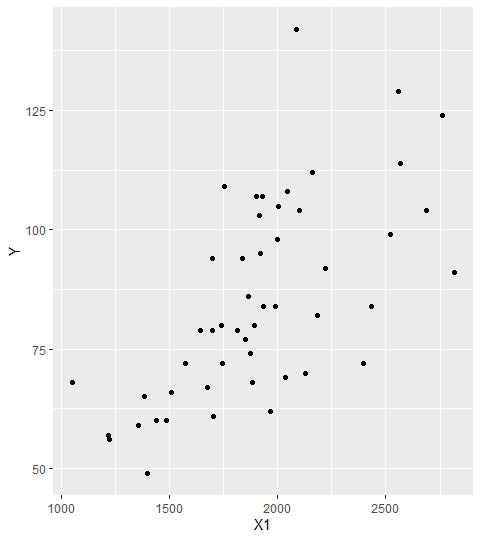
\includegraphics{Y vs X1}

\item
Please plot the relationship between \emph{Y} and \emph{Region}? On average, which region does have the highest per capita expenditure on public education?
\vspace{.5cm}
\item
Please plot the relationship between \emph{Y} and \emph{X1}? Describe this graph and the relationship. Reproduce the above graph including one more variable \emph{Region} and display different regions with different types of symbols and colors.
\end{itemize}

\end{document}
